\section{Quantization: Uniform}
\label{sec:Quantization: Uniform}

\subsection{Objective}
Computing the Signal to quantization Noise ratio of Uniform Quantization. 
Plot SNQR vs. Quantization levels.

\subsection{Theory}
The Signal to Quantization Noise Ratio (SQNR) is the ratio of the signal power to the quantization noise power.
It is defined as:

\begin{equation}
	SQNR = \frac{P_s}{P_q}
\end{equation}

where $P_s$ is the signal power and $P_q$ is the quantization noise power.

For uniform quantization, the signal power is given by:

\begin{equation}
	P_s = \frac{1}{3} \sum_{i=1}^{N} (x_i - x_{i-1})^2
\end{equation}

\subsection{Matlab Code}

\inputminted[fontsize=\footnotesize,autogobble]{matlab}{code/sqnr.m}

\subsection{Output}

\begin{figure}[!htb]
	\centering
	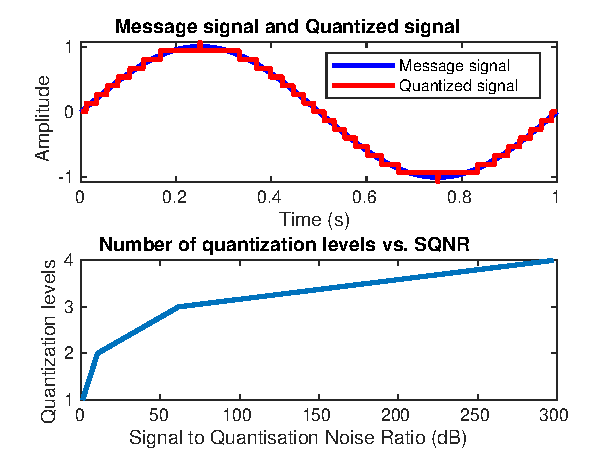
\includegraphics[width=0.70\textwidth]{res/figures/Figure_6.pdf}
	\label{output:SQNR vs quantization}
	\caption{SQNR vs Quantization}
\end{figure}

\pagebreak
\section{Quantization: Non-Uniform}
\label{sec:Quantization: Non-Uniform}

\subsection{Objective}
Computing SNR of Non-Uniform Quantization and Plot SNR vs. Quantization Levels

\subsection{Matlab Code}

\inputminted[fontsize=\footnotesize,autogobble]{matlab}{code/sqnr2.m}
\subsection{Output}

\begin{figure}[!htb]
	\centering
	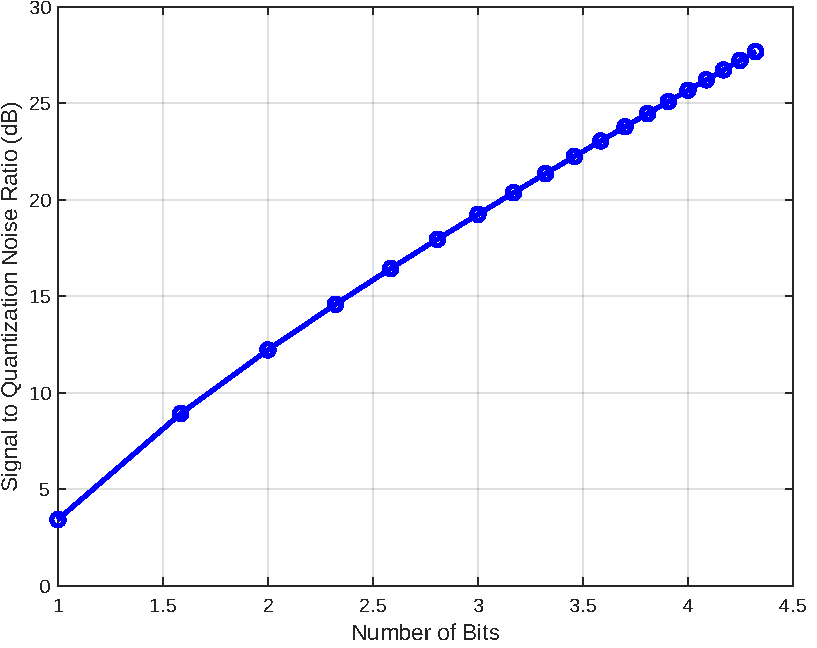
\includegraphics[width=0.7\textwidth]{res/figures/Figure_4.pdf}
	\label{output:SQNR vs quantization 2}
	\caption{SQNR vs Quantization (non-uniform)}
\end{figure}